\documentclass[12pt]{amsart}
\numberwithin{equation}{section}
\numberwithin{figure}{section}
\numberwithin{table}{section}
\usepackage{latexsym}
\usepackage{harvard}
\usepackage{lscape}
\usepackage{graphics}
\usepackage{dsfont}
\usepackage{epsfig}
\usepackage{subfigure}
\usepackage{alltt}
\font\TenCyr=wncyr10
\setcounter{secnumdepth}{3}
\setcounter{tocdepth}{3}
\setlength{\textwidth}{135mm}
\setlength{\textheight}{205mm}
\setlength{\oddsidemargin}{10mm}
\setlength{\evensidemargin}{10mm}
\setlength{\topmargin}{0mm}
\setlength{\textwidth}{6in}
\setlength{\marginparwidth}{20mm}
\DeclareMathAlphabet{\mathsi}{OT1}{cmss}{m}{sl}
%\renewcommand{\abstractname}{}
\makeatletter
%\renewcommand{\section}{\@startsection{section}{1}{0em}{1.5\baselineskip}%
%    {0em}{\centering\sffamily\normalsize\bfseries}}
\renewcommand{\section}{\@startsection{section}{1}{0mm}%
    {-0.5\baselineskip}{0.01\baselineskip}
%    {\centering\sffamily\normalsize\slshape}}
     {\centering\normalsize\bfseries}}
\renewcommand{\subsection}{\@startsection{subsection}{2}{0mm}%
    {-0.5\baselineskip}{0.01\baselineskip}
%    {\sffamily\normalsize\slshape}}
     {\normalsize\bfseries}}
\makeatother
\renewenvironment{proof}{\noindent {\bf Proof.\ }}{\hfill{ \rule{2mm}{2mm}}}
\newtheorem{ass}{Assumption}
\newtheorem{lemma}{Lemma}[section]
\newtheorem{thm}{Theorem}[section]
\newtheorem{prop}{Proposition}[section]
\def\sT{\scriptscriptstyle T}
%\def\RR{\hbox{\raise.4ex\hbox{$\scriptstyle{|}$}\hskip-1.85pt R}}
\def\RR{\mathds{R}}
\def\GG{\mathcal{G}}
\def\VV{\mathcal{V}}
\newcommand{\Trace}{\mbox{Trace}}
\newcommand{\dint}{\,d}
\newcommand{\grad}{\,\nabla\!}
\newcommand{\hess}{\,\nabla^2\!}
\newcommand{\ltwonorm}{|| \cdot ||_2}
\newcommand{\lonenorm}{|| \cdot ||_1}
\newcommand{\trans}{^{\scriptscriptstyle\mathsi{T}\unskip}}
\newcommand{\Jureckova}{Jure\v{c}kov\'{a} }
\newcommand{\Hajek}{H\'{a}jek }
\newcommand{\Hardle}{H\"{a}rdle }
\newcommand{\Sidak}{\v{S}id\'{a}k }


\begin{document}
\bibliographystyle{econometrica}



\title {\bf Penalized Triograms:\\  
Total Variation Regularization for Bivariate Smoothing}

\thanks{
Version: {\today}.
Corresponding author:  Roger Koenker, Department of Economics,
University of Illinois, Champaign, IL, 61820, USA. 
Email: roger@ysidro.econ.uiuc.edu.}



\author{Roger Koenker}
\address{University of Illinois at Urbana-Champaign }
\author{Ivan Mizera}
\address{University of Alberta }

\keywords{ Penalty methods, regularization, spline smoothing, total variation }

\begin{abstract}
\citeasnoun{HKS:1998} introduced a family of continuous, 
piecewise linear functions defined over adaptively selected triangulations of 
the plane as a general approach to statistical modeling of bivariate 
densities, regression and hazard functions.  
These {\em triograms}
enjoy a natural affine equivariance that offers distinct
advantages over competing tensor product methods that are more  
commonly used in statistical applications.


Triograms employ basis functions consisting of linear
``tent functions'' defined with respect to a triangulation of a given
planar domain.  As in knot selection for univariate splines, 
Hansen, {\it et al} adopt the regression spline approach of 
\citeasnoun{ston:1994}. 
Vertices of the triangulation are introduced or removed sequentially in an 
effort to balance fidelity to the data and parsimony. 

In this paper we explore a smoothing spline variant of the 
triogram model based on a roughness penalty
adapted to the piecewise linear structure of the triogram model. 
We show that the proposed roughness penalty may be interpreted 
as a total variation penalty
on the gradient of the fitted function.  The methods are illustrated
with both real and artificial examples, including an application to
estimated quantile   surfaces of land value in the Chicago metropolitan area.

\end{abstract}

\maketitle

\pagestyle{myheadings}
\markboth{\sc Penalized Triograms}{\sc Roger Koenker and Ivan Mizera}

\section{Introduction}

Piecewise polynomial functions, or splines, have proven to be an extremely 
powerful concept throughout approximation theory and the statistical
literature on smoothing.  Like the eponymous drafting instrument, splines are
an elegantly simple, yet eminently practical tool.
In the statistical literature on splines
there continues to be a vigorous debate over the 
relative merits of penalty methods for smoothing splines, versus 
regression splines relying on knot selection.  
Both computational tractability and statistical efficiency play important
roles in this debate, and the resulting rivalry has significantly
broadened the scope of both approaches.

\citeasnoun{HKS:1998} have recently introduced
a class of linear spline models for bivariate smoothing problems.
These triogram  models are defined on triangulations of polyhedral
planar domains.  Knot selection strategies adapted from the
regression spline methods of \citeasnoun{SHKT:1997}
are proposed to control the degree of smoothness of the estimates.
The primary objective of the present paper is  to explore a
smoothing spline approach to the estimation of triograms.  The roughness
penalty we employ may be interpreted as an extension to bivariate settings
of the total variation roughness penalty suggested in \citeasnoun{KNP:1994} 
for univariate smoothing problems.


\section{On Roughness Penalties}

In its classical univariate form the cubic smoothing spline solves
the problem of finding a function $g$ minimizing
\[
\sum_{i=1}^n (y_i - g(x_i))^2 + 
\lambda \int (g''(x))^2 dx,
\]
over a Sobolev space  of continuous functions  with
absolutely continuous first derivative and square-integrable second
derivative. The tuning parameter $\lambda$ controls the smoothness of
the fitted function. In this form the estimator $\hat g $ is
a natural cubic spline with knots at the observed $x_i$'s and may be
interpreted as an estimate of the conditional mean function. The
penalty term may be interpreted as
a prior belief that the $L_2$ norm of $g '' $ is unlikely
to exceed a specified bound controlled by the choice of $\lambda$.

\subsection{Total Variation Roughness in the One-dimensional Case}
There have been
numerous efforts to explore alternative forms of both the fidelity and
roughness penalties to achieve modified objectives. One such effort is
described in \citeasnoun{KNP:1994}, where a non-parametric approach to
estimating conditional quantile functions is suggested based on minimizing
\begin{equation}
\label{eq:qss}
\sum_{i=1}^n \rho_\tau ( y_i - g(x_i) ) + \lambda J (g),
\end{equation}
where $\rho_\tau (u) = u ( \tau - I ( u < 0))$ generates a fidelity
term appropriate for conditional quantile estimation, and the
roughness penalty $J(g)$ is taken to be the total variation of the
first derivative of $g$.  
Recall that total variation of a function $f: [a,b] \rightarrow \RR$ is given by
\[
V(f) = \sup_\pi \sum_{k=0}^{n-1} | f(x_{k+1}) -f(x_k) |
\]
where $\pi$ denotes partitions: $a \leq x_1 < x_2 < \ldots < x_n \leq b$.
\
If $g'$ is absolutely continuous, we can also write, 
(Natanson, 1974, Theorem IX.4.8), \nocite {natanson}
\begin{equation}
\label{eq.pen}
J(g) = V (g') = \int |  g''(x)| dx.
\end{equation}
This establishes a clear link between the total variation roughness penalty 
and the classical $L_2$ penalty.
For smooth functions, the total variation penalty is simply the $L_1$
analogue of the classical $L_2$ smoothing spline penalty.
\citeasnoun{MdG} have studied total variation penalties with $L_2$ fidelity
in the univariate setting; together with \citeasnoun{P.97}, 
they have explored the asymptotic behavior of related estimators.  


From a theoretical perspective, the use of total variation penalties 
enables the fit to mimic sharp bends, spikes and edges more easily than the
conventional $L_2$ penalties.  For this reason, total variation penalties
have received considerable attention in the image processing literature
dating back to \citeasnoun{ORF};  see also \citeasnoun{OR}.  
In contrast to the penalty \eqref{eq.pen},
which penalizes variation in the derivative of $\hat g$, the imaging
literature has focused primarily on variation of the function itself.
See \citeasnoun{TWBO} and \citeasnoun{Scherz98} for exceptions.
Total variation penalties applied on the function itself have been
recently considered also in the statistical literature, by \citeasnoun{nicholls}
and \citeasnoun{DK.01}. This approach permits discontinuities in
the fitted functions, and consequently is connected to
work on total variation penalties for bivariate functions
used for edge detection and segmentation in the image processing literature.  

From a more pragmatic viewpoint, total variation penalties are well matched
for the quantile regression fidelity since they preserve the linear programming
formulation of the optimization problem defining the estimator.  Solutions
to the problem \eqref{eq:qss} take the form of piecewise linear functions with 
jumps in their derivative at a few of the observed $x_i$'s.  
The $L_1$ nature of the total variation
penalty imposes a rather different shrinkage effect than the classical
$L_2$ penalty. Just as ordinary $\ell_1$ regression seeks to identify
$p$ basic observations whose exact fit characterizes the
$p$-dimensional parameter estimate, the $L_1$ penalty acts more like a
model selection device by identifying a small number of critical $x_i$
points at which $\hat g'$ will be allowed to jump. The number of these
selected jump points is controlled by the parameter $\lambda$, and
provides a natural measure of the dimensionality of the fitted.
See Section 4.7 below and \citeasnoun{tibs:1996} 
and \citeasnoun{DCS:1998} for related discussion of the 
model-selection, shrinkage effects of $L_1$ type penalties.

\subsection{Thin Plate Penalties for Bivariate Smoothing}
The extension of univariate smoothing splines to bivariate situations,
and beyond, raises new questions about how to measure the
roughness of surfaces. The thin plate smoothing splines of \citeasnoun{HD.1972}
whose theory was developed by Duchon
(1976,1977),\nocite{Duc76,Duc77} \citeasnoun{meinguet:1979}, 
\citeasnoun{WahWen80}, and others, minimize
\begin{equation}
\sum_{i=1}^n (z_i - g(x_i , y_i ))^2 + \lambda J(g, \varOmega,  \| \cdot  \|_2^2 ),
\label{eq.thinp}
\end{equation}
with the roughness penalty defined as
\begin{equation}
\label{eq.tp}
J(g,\varOmega, \| \cdot  \|_2^2) = 
	\iint_{\varOmega}  \| \hess g  \|_2^2 dxdy =
	\iint_{\varOmega} ( g_{xx}^2 + 2 g_{xy}^2 + g_{yy}^2 )dxdy.
\end{equation} 
A considerable simplification is achieved in the
classical form of thin-plate setting, when $\varOmega$ is taken to be
all of $\RR^2$; however, as noted by \citeasnoun{gree:silv:1994},
there can be considerable disparities between such solutions and
solutions based on versions of the penalty defined over restricted
domains.  


If $g(x,y) = h(x)$ for some $h$, then a straightforward computation
shows that, on rectangular $\varOmega = \varOmega_1 \times \varOmega_2$,
\begin{equation}
\label{eq.redu}
J(g,\varOmega, \ltwonorm^2) = J(h,\varOmega_1,\ltwonorm^2) \ \mu( \varOmega_2),
\end{equation}
where $ J(h,\varOmega_1,\ltwonorm^2)$ specializes to the classical
univariate penalty $\int (g'' (x))^2 dx$, and 
$\mu(\varOmega_2)$ denotes the Lebesgue measure of
$\varOmega_2$. Thus, the thin plate penalty \eqref{eq.thinp} may be
viewed as a natural bivariate extension of the classical univariate
roughness penalty. This raises the following questions. Can we,
by analogy with the univariate total variation penalty \eqref{eq.pen},
define a bivariate roughness penalty? How should we define total variation of
the gradient of a function of two variables? 

\subsection{Total Variation in Higher Dimensions}
The quest for a satisfactory definition of total variation for
functions from $\RR^k$ to $\RR^m$ has engaged the mathematical
community for more than a century. Only for $k=1$, and $m$ arbitrary,
does the classical univariate definition of
\citeasnoun{Jor81} adapt in a straightforward way, see
\citeasnoun{Din67}. Early definitions for $k \geq 2$ and $m=1$ by
Tonelli (1926, 1936), \nocite{Ton26,Ton36} and others suffered from
coordinate-dependence and attendant reliance on rectangular
domains---a drawback in nonparametric regression, as we argue below.
The first orthogonally-invariant definitions were introduced by
Kronrod (1949, 1950) \nocite{Kro49,Kro50} in the spirit of the Banach
indicatrix theorem. However, eventually the approach based on the
Vitali formula interpreted in the language of Schwartzian distribution
prevailed; \citeasnoun{AmbFusPal00} give a recent account of the theory
developed in the context of geometric measure theory and variational
calculus, tracing its origins back to \citeasnoun{Fic54} and
\citeasnoun{Gio54}.

As in the theory of Sobolev spaces, the formalism of distributions is
needed only for differentiation and limit transitions; the functions
under consideration remain standard. A convenient initial step is to
outline the functional domain in a qualitative way, without recourse
to any particular total variation functional. Functions with bounded
variation are defined to be those whose derivatives, in the sense of
distributions, are measures. The defined functions
encompass not only smooth functions with bounded variation, but also,
for instance, piecewise linear or piecewise constant, that is, discontinuous,
functions with bounded variation. For a smooth function $f$ from
$\RR^k$ to $\RR^m$, we define
\begin{equation}
\label{eq.defvar}
V (f, \varOmega, \|\cdot\|)
        = \int_\varOmega \| \grad f \| \dint x;
\end{equation}
here $\dint x$ denotes (multiple) integration with respect to
$k$-dimensional Lebesgue measure. The functional $V$, initially
defined for smooth functions, is lower semicontinuous, and so it can be
extended to a broader domain via the approach of \citeasnoun{Ser61}:
\begin{equation}
\label{eq.defser}
V(f) = \liminf V(f^\nu),
\end{equation}
where the right-hand side expression denotes the infimum of $\liminf
V(f^\nu)$ over all sequences $f^\nu$ approaching $f$ in the sense of
distributions. It can be shown that the extended $V$ assigns a finite
value to every function with bounded variation; that is, the extension
is nontrivial.
 
For a function $g$ from $\RR^2$ to $\RR$ we thus define a penalty
\begin{equation}
\label{eq.defpen2}
J(g, \varOmega, \| \cdot \|) =
V(\grad g, \varOmega, \| \cdot \|) =
\iint_\varOmega \| \hess g \| \dint x \dint y.
\end{equation}
This penalty assigns a finite value to every function whose gradient
has bounded variation---in particular, to every piecewise-linear
continuous function on bounded domains with finite number of linear
pieces. This is in contrast with the behavior of the thin-plate
functional \eqref{eq.tp}.  Since the latter is also lower semicontinuous,
one may contemplate an extension analogous to \eqref{eq.defser} also for
this functional.  However, as shown by \citeasnoun{Ser61},
any such an extension assigns $+\infty$ to any $f$ with discontinuous
derivatives; in particular, any function with a spike or a sharp ridge
is evaluated as infinitely rough.
 
Any penalty of the form \eqref{eq.defpen2} can be considered an
extension of the univariate penalty \eqref{eq.pen}, regardless of the
choice of the norm.
\begin{thm}
\label{thm1}
Suppose that $g$ is a function from $\RR^2$ to $\RR$ such that
$g(x,y) = h(x) + ky$ for some $h:\RR \rightarrow \RR$ and real value $k$.
There is a constant $c$ depending only
on the choice of the matrix norm in \eqref{eq.defpen2}, but not on $g$,
such that for any $\varOmega = \varOmega_x \times \varOmega_y$,
\begin{equation}
\label{eq:thm1}
J(g,\varOmega, \| \cdot \|) = c\, J(h,\varOmega_x, \| \cdot \|) \
|\varOmega_y|,\end{equation}
where
$J(h,\varOmega_x, \| \cdot \|) = \int_{\Omega_x} |h'' (x) | \dint x$, and
$|\varOmega_y|$ denotes the Lebesgue measure of $\varOmega_y$.
\end{thm}
\begin{proof}
Let $c$ be the norm of the $2 \times 2$ matrix containing $1$ in the upper
left corner and zeros elsewhere. By the properties of the
norm, the norm of the matrix containing $u$ instead of $1$ in the
upper left corner and zeros otherwise is $c |u|$. Note that in the
Hessian, all second-order partial derivatives are zero, except for
$g_{xx} (x,y)= h''(x)$; thus
\begin{equation*}
J(g,\varOmega, \| \cdot \|) = c \iint_{\varOmega}  | h''(x) | \dint x \dint y
\end{equation*}
and \eqref{eq:thm1} follows by the Fubini theorem for all smooth $g$
and hence by extension for all $g$ under consideration.
\end{proof}


 
\subsection{The Choice of the Norm: Invariance and Equivariance}
 
For denoising images with a view toward reconstructing discontinuities in
derivatives, \citeasnoun{Scherz98} proposed using the penalty corresponding
to the $\ell_1$ norm in \eqref{eq.defvar}; for smooth functions $g$
from $\RR^2$ to $\RR$ this penalty is equal to
\begin{equation}
\label{eq.stv}
J(g, \varOmega, \| \cdot \|_1 )
        = \iint (| g_{xx} | + 2 | g_{xy}| + | g_{yy} |) dx dy.
\end{equation}
A related penalty has been recently proposed in the statistical literature by
\citeasnoun{HNP:1998}, who introduced a bivariate form of the
quantile smoothing spline using a roughness penalty that sums
univariate total variation of the function along rectangular grid
lines. Their roughness penalty may be viewed as a total variation of
the gradient in the Tonelli--Cesari vein of \eqref{eq.defvar}, with the
$\ell_1$ norm applied to the diagonal of the Hessian,
\begin{equation}
\label{eq.hnptv}
J(g, \varOmega, \| \cdot \|_{HNP})
        = \iint ( | g_{xx} | + | g_{yy} | ) dx dy.
\end{equation}
Their formulation
gives rise to bilinear tensor product splines that are continuous and
piecewise linear on the grid lines, and bilinear on the rectangular
patches between grid lines. Similar tensor product splines have also
been widely used in the least-squares regression spline literature.
 
One potential disadvantage of the tensor product formulation
is its lack of orthogonal equivariance. Functions well
oriented with respect to the $xy$-axes may prove to be much more
difficult to fit when the observations are rotated. Invariance
considerations, as stressed by \citeasnoun{gree:silv:1994}, provide
valuable guidance through the forest of potential definitions 
of roughness penalty functionals.

The requirement of orthogonal invariance for the penalty $J$ leads
to the condition
\begin{equation}
\label{eq:uhu}
\| U\trans H U \| = \| H \|,
\end{equation}
satisfied by any orthogonal matrix $U$ and any symmetric matrix $H$.
There are many norms satisfying this property---apparently any norm
which is a symmetric function of the eigenvalues satisfies
\eqref{eq:uhu}.
The leading example of such a norm is the Hilbert--Schmidt (Frobenius,
Euclidean) norm of the matrix. The resulting penalty is, for
sufficiently smooth $g$, given by
\begin{equation*}
J(g, \varOmega, \| \cdot \|_2) = \int_\varOmega
        \sqrt{g^2_{xx} + 2g^2_{xy} + g^2_{yy}} \dint x \dint y.
\end{equation*}
Other possibilities include the spectral norm, the maximal absolute
value of the eigenvalues, or absolute value of the trace.
 
Another attractive property of total variation roughness penalties,
particularly when paired with absolute error fidelity, is their scale
equivariance. If $g$ minimizes
\begin{equation}
\label{eq:abs}
\sum_{i=1}^n |z_i - g(x_i,y_i)| + \lambda J(g,\varOmega, \| \cdot \|)
\end{equation}
then $cg$ minimizes \eqref{eq:abs} with $z_i$ replaced by $cz_i$, provided
that $J(cg,\varOmega, \| \cdot \|) = |c| J(g,\varOmega, \| \cdot \|)$.
This is clearly not the case for the thin-plate penalty,  but
for Gaussian fidelity the thin plate penalty {\it is} well matched in
this sense.



\section{Triograms}

Efficient numerical solution of the variational problems arising from
general forms of roughness penalties based on total variation
appears quite challenging. However, by restricting the domain of
functions over which we are optimizing some progress can be made. One
such restriction leads to penalized versions of the piecewise linear
triograms of \citeasnoun{HKS:1998}.

Let ${\mathcal U}$ be a
compact region of the plane, and let $\Delta$ denote a collection of
sets $\{ \delta_i: i=1, \ldots, N \}$ with disjoint interiors such that
${\mathcal U} = \cup_{\delta\in \Delta} \delta.$ In general the
collection $\Delta$ is called a tessellation of ${\mathcal U}$. We
will be concerned only with the case that the $\delta\in\Delta$ are
planar triangles, in which case $\Delta$ is called a triangulation. 
The continuous functions $g$ on ${\mathcal U}$ that are linear when
restricted to $\delta\in\Delta$ are called triograms. Their collection
${\mathcal G}$ associated with the triangulation $\Delta$ is a
finite-dimensional linear space.


\subsection{A Roughness Penalty for Triograms}



As already pointed out, thin-plate penalties are inappropriate for
triograms, since their penalties assign infinity to any function with a
discontinuity in the gradient, and thus the thin plate penalty is
inherently incapable of discriminating among triograms.
Roughness penalties based on the total variation of the gradient are
more promising.  Fortuitously, it also turns out that the troublesome choice of a norm
disappears; once we insist on a orthogonally invariant penalty for
triograms, all penalties coalesce.


\begin{thm}
\label{thm2}
Suppose that $g: \RR^2 \to \RR$
is a piecewise-linear function on the triangulation $\Delta$.
For any  orthogonally invariant penalty of the form \eqref{eq.defpen2}, there
is a constant $c$ dependent only on the choice of the norm such that,
\begin{equation}
\label{eq.basform}
J(g, \varOmega,\| \cdot \|) = 
c \sum_{k} | \nabla g^+_{e_k} - \nabla g^-_{e_k} |_2 \; | e_k |_2,
\end{equation}
where $k$ runs over all the interior edges of the triangulation,
$|e_k |_2$ is the Euclidean length of the edge $e_k $, and 
$| \nabla g^+_{e_k}  - \nabla g^-_{e_k}  |_2$ is the Euclidean length of the
difference between gradients of $g$ on the triangles adjacent to $e_k $.
\end{thm}
\begin{proof}
Evaluating $J$, we split the integration domain $\varOmega$ into
disjoint pieces whose contribution to $J$ is determined separately.
First, the contribution of all linear parts, the interiors of the
triangles, is zero; the second derivatives vanish thereon.
 
The contribution of an edge $e$ is the corresponding term in
\eqref{eq.basform}: consider the quadrilateral region consisting of two
triangles adjacent to the edge. Extend the functions on the triangles
linearly to have a rectangular domain---this should not alter the
penalty. Coordinatewise independence then allows for rotating the
rectangle so that its edges are parallel to $xy$-axes; the application
of Theorem~\ref{thm1} then gives the desired result.  

The final, and only technical part of the proof is to show that the
contribution of any vertex of the triangulation is zero. This is done
employing the definition \eqref{eq.defser}.  The sequence $g^\nu$
approximating $g$ is obtained via mollification: $g^\nu$ is taken to
be the convolution of $g$ with $\nu^2 \phi(\nu x, \nu y)$, where
$\phi$ is a smooth function assigning $0$ to all values outside the
unit circle whose integral is equal to $1$.  A common example of
such a $\phi(x,y)$ is a multiple of
$\exp (-1/(1-x^2-y^2))$ on the unit circle and $0$ elsewhere. 
When $\nu \to \infty$, $g^\nu$
approaches $g$ in the distributional sense. The contribution of the
vertex is bounded from above by
\begin{equation}
\label{eq.pf}
\liminf_{\nu \to \infty} \iint_{B_\nu} \| \hess g^\nu \| \dint x \dint y,
\end{equation}
where $B_\nu$ is the circle centered at the vertex with radius
$1/\nu$. Since any two norms on a finite-dimensional vector space are
equivalent, \eqref{eq.pf} is bounded from above by a constant multiple
of \eqref{eq.pf} with the Hilbert--Schmidt norm, the constant depending
only on the original norm. In what follows, $C$ stands for a generic
constant. Since the derivatives of $g$ in the neighborhood of the
vertex are piecewise constant, with finitely many pieces, we have
\begin{equation*}
\begin{split}
| g^\nu_{xx} (x,y) | &= 
	\left| \iint  \nu^3 
	\phi_x(\nu u, \nu v) 
	g_x (x-u, y-v) \dint u \dint v \right|
\\
&\leq \nu \iint \left| \nu^2 
	\phi_x(\nu u, \nu v) 
	g_x (x-u, y-v) \right| \dint u \dint v
\\
&\leq \nu \iint C 
	\left| \nu^2 \phi_x(\nu u, \nu v) \right| \dint u \dint v
\leq C \nu \iint  
	\left| \phi_x(u, v) \right| \dint u \dint v = C \nu;
\end{split}
\end{equation*}
the same inequalities hold for the other terms in the Hessian $\hess
g^\nu$, the constants being independent of $x$, $y$, and $\nu$. By the
properties of the Hilbert--Schmidt norm,   
\begin{equation*}
\iint_{B_\nu} \| \hess g^\nu \| \dint x \dint y
\leq \iint_{B_\nu} C \nu \dint x \dint y = C \nu^{-1}.
\end{equation*}
The last term goes to $0$ when $\nu \to \infty$. Note that for the
thin-plate penalty the bound for the elements of the Hessian would be
$C \nu^2$, and the contribution of the vertex would not vanish, though
it would be finite.  
\end{proof}
\vspace{5mm}

The crucial consequence of Theorem~\ref{thm2} is that, from the
variational point of view, there is only one viable form of the total
variation penalty penalizing the gradient of triograms: that given by
formula \eqref{eq.basform}. Penalized quantile triograms, functions minimizing
\begin{equation}
\label{eq.pentri}
\sum_{i=1}^n \rho_\tau (z_i - g(x_i , y_i )) 
+ \lambda J(g, \varOmega,\| \cdot \|)
\end{equation}
over the space of triograms $\GG$ can be then found as a solution of a
linear programming problem, as we show in the next section.


\section{Computation of Penalized Triograms}

Modern linear programming methods provide an extremely efficient means of
solving for penalized triogram estimators.  We will briefly describe how to
express elements of the linear space $\GG$ in terms of a finite set of
basis functions, and then show how the fidelity and penalty terms can be
written as piecewise linear functions of the coefficients of this expansion.
This leads to a linear programming formulation of \eqref{eq.pentri}
for which interior point, log-barrier methods exploiting the sparsity
of the linear algebra offer an efficient solution strategy.

\subsection{A Basis for ${\mathcal G}$}
A basis for the linear space ${\mathcal G}$ consists of the linear ``tent''
functions, $\{B_i(u)\}_{i=1}^p$, that may be expressed  
in terms of the barycentric coordinates of points $u$
represented by the vertices $v_1, v_2, v_3$ of the triangle $\delta$
containing $u$,
$$
u_j=\sum_{i=1}^3 B_i(u) v_{ij} \quad j=1,2.
$$
and satisfying the conditions that $0\leq B_i(u) \leq 1$ with
$$
1=\sum_{i=1}^3 B_i(u).
$$
Solving for the $B_i(u)$'s we obtain by Cramer's rule, provided the
vertices are not collinear,
$$
B_1(u) = \frac{A  (u, v_2, v_3)}{A  (v_1, v_2, v_3)},
$$
where
$$
A  (v_1, v_2, v_3) = \frac{1}{2} \left| \begin{array}{ccc}
v_{11} & v_{21} & v_{31} \\
v_{12} & v_{22} & v_{32} \\
1 & 1 & 1 \end{array} \right|
$$
is the signed area of the triangle $\delta$. The remaining $B_i(u)$
are defined analogously by replacing the vertex $v_i$ by $u$. Clearly,
the $\{B_i(u)\}$ are linear in $u$ on $\delta$, and satisfy the
interpolation conditions that $B_i(v_j) = 1$ for $i=j$ and $=0$
otherwise; thus they are linearly independent. They are also affine
equivariant; that is, for any non-singular, $2 \times 2$ matrix $A$,
and vector $b\in \RR^2$,
$$
B_i(u) = B_i^*(Au+b), \qquad u\in {\mathcal U},
$$
where $\{B_i(u)\}$ are formed from the vertices $\{v_i\}_{i=1}^p$ and
$\{B_i^*\}$ are formed from the vertices $\{A v_i+b\}_{i=1}^n$. In
particular, the basis is equivariant to rotations of the coordinate
axes, a property notably missing in many other bivariate smoothing
methods. 

\subsection{Computing the Fidelity}
Any function $g \in \GG$ may be expressed in
terms of the barycentric basis functions and the values $\beta_i$
that it takes at the vertices of the triangulation as:
\[
g(x,y) = \sum_{i=1}^p \beta_i B_i (x,y).
\]
Thus, we can express the fidelity of the function, $\hat g (x,y)$, fitted to
the observed sample, $\{ ( x_i, y_i, z_i ), i=1,...,n \}$ in $\ell_1$
terms as
\[
\sum_{i=1}^n |z_i - \hat g (x_i, y_i ) | = \sum_{i=1}^n
|z_i - a_i \trans \hat \beta |, 
\]
where the $p$-vectors $a_i$ denote the ``design'' vectors with
elements, $a_{ij} = (B_j (x_i,y_i))$.  In the simplest case
there is a vertex at every point $(x_i , y_i)$
and the matrix $A = (a_{ij})$ is just the $n$-dimensional identity.
However, one may wish to choose $p < n$ and there would be
a need to compute some nontrivial barycentric coordinates for some elements of
the matrix $A$.


\subsection{Computing the Penalty}
Fix the triangulation $\Delta$ and consider the triogram $g \in \GG$
on a specified triangle $\delta \in \Delta$.  
Let $\{ ( x_i,y_i,z_i ), \; i=1,2,3 \}$
denote the points at the three vertices of $\delta$.  We have
\[
z_i = \theta_0 + \theta_1 x_i + \theta_2 y_i \quad \quad i=1,2,3,
\]
where $\theta$ denotes a vector normal to the plane representing the
triogram restricted to $\delta$.  Solving the linear system, we obtain
the gradient vector,
\[
\nabla g_{\delta} = 
\left( \begin{array}{c}\theta_1 \\ \theta_2 \end{array} \right)
= [\text{det}(D)]^{-1}
\left( \begin{array}{ccc}
(y_2 - y_3) & (y_3 - y_1) & (y_1 - y_2) \\
(x_3 - x_2) & (x_1 - x_3) & (x_2 - x_1) 
\end{array} \right)
 \left( \begin{array}{c}z_1 \\ z_2 \\ z_3 \end{array} \right),
\]
where $D$ is the 3 by 3 matrix with columns $[ 1, x, y ]$.
This gradient is obviously constant on $\delta$ and linear in the values of
the function at the vertices.  Thus, for any pair of triangles
$\delta_i , \delta_j$ with common edge $e_{k(i,j)}$ we have the
constant gradients $\nabla g_{\delta_i}, \nabla g_{\delta_j}$ and we
can define the contribution of the edge to the total roughness of
the function as
\[
| c_k | = | \eta_{ij} \trans (\nabla g_{\delta_i} - \nabla g_{\delta_j} ) |
\; \cdot  | e_{k(i,j)}  |_2
=  | (\nabla g_{\delta_i} - \nabla g_{\delta_j} )  |_2
\; \cdot  |  e_{k(i,j)}  |_2,
\]
where $\eta_{ij}$ denotes the unit vector orthogonal to the edge.
The second formulation follows from the fact that $\eta_{ij}$ is
just the gradient gap renormalized to have unit length; this
can be easily seen by considering a canonical orientation in which
the edge $k(i,j)$ runs from $(0,0)$ to $(1,0)$.
The penalty is then computed by summing these contributions over
all interior edges.

Since the gradient terms are linear in the 
parameters $\beta_i$
determining the function at the vertices, the penalty may also be 
expressed as a piecewise linear function of these values, i.e.,
\[
\sum_{k=1}^M |c_k | = \sum_{k=1}^M | h_k \trans \hat \beta |,
\]
where the index $k$ runs over all of the $M$ edges formed by the triangulation
$\Delta$.  
The problem of optimizing the fidelity of the fitted function subject to a 
constraint on the roughness of the function may thus be formulated as
an augmented linear $\ell_1$ problem minimizing
\begin{equation}
\sum_{i=1}^n |z_i -a_i \trans \beta | + \lambda \sum_{k=1}^M |h_k \trans \beta|.
\label{eq.augtri}
\end{equation}
This approach to estimating penalized median surfaces may be immediately
extended to estimation of penalized quantile surfaces by minimizing
\begin{equation}
\sum_{i=1}^n \rho_\tau (z_i -a_i \trans \beta ) + 
\lambda \sum_{k=1}^M |h_k \trans \beta|.
\label{eq.augtrirq}
\end{equation}


\subsection{Penalized Triograms for Conditional Mean Models}
A corresponding penalized least squares problem may be formulated to minimize
\begin{equation}
\sum_{i=1}^n (z_i -a_i \trans \beta )^2 + \lambda \sum_{k=1}^M (h_k \trans \beta )^2.
\label{eq.l2tri}
\end{equation}
Like the median regression problem this may be viewed as an augmented
regression problem with response vector
$(z \trans,0 \trans) \in \RR^{n+M}$, and design
matrix $[A
\trans \vdots H \trans ] \trans $ where $A = (a_i \trans )$ and
$H=(h_k \trans )$.
This $L_2$ variant of penalized triogram has been explored further by 
\citeasnoun{HK.02}. 
It may be noted that the primal-dual interior point methods used to
minimize (4.1) begin their iterations by solving (4.3),
and continue to take iteratively reweighted least squares
steps until a solution is reached with at least $p$ zero residuals.
Thus \eqref{eq.l2tri}, although not covered by \eqref{eq.defpen2}, 
can be viewed as leading to a one-step version of the
total variation penalized triogram.


\subsection{Penalized Triograms as Linear Programs}

The problem \eqref{eq.augtri} is piecewise linear in $\beta$, so it
is straightforward to reformulate it as a linear program.  Let
\[
X = \left[ \begin{array}{c} A \\ \lambda H \end{array} \right] ,
\]
where $A$ denotes the matrix with rows $(a_i \trans )_{i=1}^n$ and
$ H = (h_i \trans)_{i=1}^M$, and denote the augmented response vector as 
$\zeta = (z \trans , 0 \trans ) \trans$.  The problem \eqref{eq.augtri} 
of minimizing the $\ell_1$ norm of the vector $\zeta - X\beta$ 
may be expressed as
\begin{equation}
\label{eq.lpform}
\min_{(\beta,u,v)} \{ 
1 \trans u +
1 \trans v | \zeta = X\beta +u -v, \; \beta \in \RR^p, u \geq 0, v \geq 0 \}.
\end{equation}
Hence we are minimizing a linear function subject to linear equality and
inequality constraints.  The simplex algorithm provides
an efficient solution method for moderate size problems of this type, 
but recent development of interior point methods provide an effective 
strategy even for  extremely large problems.  In effect, the interior point 
approach replaces the inequality constraints by a logarithmic barrier 
penalty function, and rather than traversing outside edges of the 
constraint set, it takes Newton type steps from the interior of the
constraint set toward the boundary solution.  See \citeasnoun{PK.1997}
for a detailed discussion.

A salient feature of the polyhedral structure of the underlying
optimization is that solutions can be characterized by a set of
``basic variables''. In the present case this basic set, $h$, consists
of $p$ elements of the first $n+M$ integers. Solutions may be written
as
\[
\hat \beta (h) = X(h)^{-1} \zeta (h),
\]
where $X(h)$ denotes the $p$ by $p$ submatrix of $X$ with rows indexed by $h$,
and $\zeta (h)$ denotes the $p$ corresponding elements of $\zeta$.
When multiple solutions exist they constitute a convex polyhedral set
with solutions of the form $\hat \beta (h)$ as extreme points.
Some of the rows of $X(h)$ will be drawn from the upper $A$ part of the
$X$ matrix, and some will come from the lower, $\lambda H$ part. If we
now evaluate the fit at the $n$ observed points we have
\[
(\hat g (x_i))_{i=1}^n = A X(h)^{-1}\zeta (h).
\]
For any element $i \in h$, the product $x_i \trans X(h)^{-1}$ is a
unit basis vector $e_j$ such that $x_i \trans X(h)^{-1} \zeta (h) =e_j
\trans \zeta (h) = \zeta_i$. When $i$ comes the first $n$ integers, so
$x_i$ is a row of $A$, this implies that the $i$th data point is
interpolated, since for these points $\zeta_i = z_i$. When $i$ comes
from the set $\{ n+1, ... , n+M\}$ the $i$th fitted value is
determined by the contribution of the penalty part of the $X$ matrix,
in conjunction with the interpolated points. Thus, only a subset of
the $n$ observations, say $p_\lambda$ of them, are needed to describe
the fit. Of course {\it all} of the observations are needed to
determine {\it which} observations are interpolated, but once the fit
is found, it can be described completely if one knows the $p_\lambda$
points that are interpolated, the triangulation, and the value of
$\lambda$. We will interpret $p_\lambda$ as an effective dimension of the
fitted model. As $\lambda$ increases, $p_\lambda$ decreases; near
$\lambda = 0$ all of the observed points are interpolated, and for
sufficiently large $\lambda$ only the three points necessary to determine
the best fitting ``median plane'' need to be interpolated.



\subsection{On Sparsity}

A crucial feature of the penalized triogram estimators described above
is the sparsity of the augmented design matrices.  In the fidelity 
component $A$, rows have at most three non-zero elements needed to
represent the barycentric coordinates of the $(x_i , y_i)$ points not
included as vertices of the triangulation.  
For observations whose $(x_i,y_i)$ points are included as vertices of
the triangulation, the vector $a_i$ is one
in only one element and zero everywhere else.  In the penalty matrix $H$, 
each row has four nonzero entries corresponding to the contribution of the
four vertices of the quadrilateral corresponding to each edge.
The remaining elements of each $h_k$ row are zero.
This sparsity of the  design matrix contrasts sharply with the situation for
thin plate splines where the corresponding matrices for the penalty
component are dense.

To appreciate the consequences of this it may help to consider an example.
Suppose we have $n=1600$ observations and we introduce vertices 
at each of the points, $\{ (x_i , y_i ): i = 1, ... , n\}$. 
The resulting matrix $A$ is just an identity matrix of dimension $n=1600$. 
The
number of interior edges of the Delaunay triangulation is given by
$e = 3 n - 2 c - 3$,
where $c$ denotes the number of exterior edges,  see \citeasnoun{OBSC}.
So the matrix $H$ is 4753 by 1600 in a typical example, and the augmented 
$\ell_1$ regression
problem is thus, 6353 by 1600.  This may at first sight
appear computationally intractable,
and would be intractable on most machines using conventional statistical
software. But recognizing the sparsity of the problem, that is, noting
that only 0.2 percent of the more than 10 million
elements of the design matrix are nonzero, reduces the memory
requirement  and computational complexity of the problem from about 80Mb
to only 160Kb.

In our Matlab and R implementations only
the nonzero elements of the design matrix are stored, along
with their identifying indices. This drastically reduces the memory
requirements of the computations and improves efficiency. As we note
more explicitly below, fitting our penalized quantile triograms
requires only a few seconds for our smaller examples, and up to about
a minute on the larger ones in our Matlab implementation. Much better
performance is attained in R where the computations are recoded in fortran
using widely available sparse matrix libraries.  See \citeasnoun{KN.02}
for details.

\subsection{Automatic $\lambda$ Selection}

Despite numerous reservations expressed in the literature about
over-reliance on automatic methods for selecting smoothing parameters,
regularization methods not confronting the problem of
selecting $\lambda$ would be considered incomplete.  A
full discussion of this deep and delicate subject is beyond 
our present scope;  instead, we mention several approaches that
we have considered in the course of our investigations. 

\citeasnoun{ORF} propose a discrepancy method, 
choosing $\lambda$ to match a preselected
fidelity value.  We employ this method in our first example in the 
next section where we choose  
$\lambda$ to match the fidelity achieved by  other smoothing method. 
See \citeasnoun{Wah90} for further comments on this approach.   

One can also base a $\lambda$
selection criterion on a reasonable measure for the effective
dimension of a fit $\hat g_\lambda $ for given
$\lambda$. As with other $\ell_1$ type estimation methods, such a
measure is provided by simply counting the number $p_\lambda$ of
interpolated observations in the fidelity component of objective
function. The recent work of \citeasnoun{MW.00} gives an additional
support for this choice---they consider the divergence,
\[ 
\mbox{div} ( \hat g) = \sum \frac{\partial}{\partial y_i} \hat g (x_i)
\]
as a general measure of effective dimension for nonparametric
regression. For linear estimators this measure yields the trace of the
corresponding linear operator, which has been suggested for classical
smoothing splines by several other authors. 
The complementary quantity, $n$ minus the effective dimension, is sometimes
referred to as ``equivalent degrees of freedom.''
For monotone regression
estimation, \citeasnoun{MW.00} show that the pool adjacent violators
algorithm yields a piecewise constant estimate, $\hat g$ with
$\mbox{div} (\hat g)$ equal to the number of distinct values taken by
$\hat g$. For our total variation penalized quantile triograms
$\mbox{div} (\hat g) = p_\lambda$ the number of points interpolated by
$\hat g$, a fact that follows from the concluding comments of Section
4.5.

Once the effective dimension, $p_\lambda$, of the fit is defined, 
it can be plugged into any of the well-known model selection criterion.
\citeasnoun{KNP:1994} suggest using the \citeasnoun{schw:1978} criterion in
their one-dimensional context. In our setting SIC selects $\lambda$ minimizing
\[
SIC(\lambda) = \log ( n^{-1}
\sum \rho_\tau (z_i - \hat g_\lambda (x_i , y_i )) ) + 
.5 n^{-1} p_\lambda \log n.
\]
Analogously, we may define a version of the Akaike criterion 
\[
AIC(\lambda) = \log ( n^{-1}
\sum \rho_\tau (z_i - \hat g_\lambda (x_i , y_i )) ) + 
n^{-1} p_\lambda.
\]
and there are certainly other possible uses for $p_\lambda$ in this vein.


Rather than simply counting the number of observations in the fidelity
component with absolute residuals smaller than a specified tolerance,
$p_\lambda$ can be obtained by computing the trace of the hat matrix
in the final weighted least squares step of the interior point algorithm.
This approach has the added advantage that it suggests a 
linearized form of the generalized cross-validation criterion that can be
used for $\lambda$ selection.
Finally, classical cross-validation is also entirely feasible in small to 
moderate size problems, and further work on computational shortcuts may be able
to extend the range of applicability of these methods.

\subsection{On Triangulations}

Up to this point we have taken the form of the triangulation, $\Delta$,
as fixed.  We now consider how to determine $\Delta$
given the observations, $\{ (x_i,y_i,z_i), \; i=1,...,n \}$.
In full generality, as we have already suggested,
this is an extremely challenging problem that involves
a delicate consideration of the function being estimated.  This draws us
back into vertex insertion/deletion schemes like those described by Hansen,
Kooperberg, and Sardy.  Since it was our intention from
the beginning to circumvent these
aspects of the problem, replacing such model selection strategies by
shrinkage governed by our proposed roughness penalty, we will focus on
the classical triangulation method of Delaunay.

A simple, direct characterization of the Delaunay triangulation may be stated for points in general
position in the plane.  We will say that points in $\RR^2$ are in general 
position if no three points lie on a line, and no four points lie on a circle.
The Delaunay triangulation of a set of points 
$\VV = \{ v_i \in \RR^2 :  i=1,...n \}$ in general
position consists of all triangles whose circumscribing circle contains
no $\VV$-points in their interior.  
There is a vast literature on how to compute the Delaunay triangulation.  

Another way to characterize the Delaunay triangulation is that it maximizes
the minimum angle occurring in the triangulation.
This maxmin property was long considered a major
virtue of the Delaunay method for reasons of numerical stability.  
Relatively recently, however,  it has 
been noted by \citeasnoun{rippa:1992} that the benefits 
of this prejudice against long, thin triangles
depend upon the eventual application of the
triangulation.  If, for example, the objective is to find a good
interpolant for a function whose curvature happens to 
be  very large in one direction
and small in the other, then long thin triangles may be very 
advantageous.
  
The sensitivity of the approximation quality to the choice of the
triangulations suggests the need for careful selection, especially if a
small number of vertices are employed.  An advantage of penalty
methods in this respect is that their reliance on a considerably larger
set of vertices can compensate to some degree for deficiencies in the
triangulation. One may restrict attention to Delaunay triangulations based 
on the observed $(x,y)$ points, but it is straightforward to incorporate
``dummy vertices'' at other points in the plane, vertices that contribute
to the penalty term, but not to the fidelity. 
By so doing one can possibly ameliorate the effect of the initial
triangulation and refine the fit to achieve more flexibility.   This
approach works in practice and is illustrated in the treatment of the
examples.  Such ``mesh refinement'' strategies have an extensive history
in the finite element literature and constitute an interesting
theoretical challenge for future investigation, in particular questions
about limit behavior and dependence on the sampling strategy.



\subsection{Boundary and Qualitative Constraints}
A triogram is convex if and only if it is convex on all pairs of adjacent
triangles.  This condition is easily checked for each quadrilateral since it
reduces to checking a linear inequality on the values taken by the
function at the four vertices of the quadrilateral.  Imposing convexity
on penalized triogram fitting thus amounts to adding $m$ linear inequality
constraints to the problems already introduced, where $m$ denotes the
number of interior edges of the triangulation.  This is particularly
straightforward in the case of the quantile fidelity given the linear
programming formulation of the optimization problem.
Similarly, it is straight forward to impose constraints 
on the boundary of the fitted surface if prior information about how
to treat these edges is available.


\section{Examples}


\subsection{Cobar mining data}

The first example employs data consisting of 38
measurements on the ``true width'' of an ore-bearing rock layer from a
mine in Cobar, Australia. These data have been analyzed
with two types of thin-plate penalty methods in 
\citeasnoun{gree:silv:1994}; we refer interested readers
to their analyses and figures for comparisons. Like Green
and Silverman, we do not employ an automatic method for $\lambda$
selection, but rather provide two exploratory fits for different $\lambda$, to
illustrate the virtues of the smoothing method. We selected two
$\lambda$'s yielding the same ($\ell_2$) fidelity for our fits as 
that achieved by Green and Silverman for their two reported fits, 
an interpolatory and a smoothing one.  The contour plots of the
two fits are illustrated in Figure 5.1.
The plot on the left interpolates all 38 of the observed points and corresponds
to $\lambda = .001$, while the right plot interpolates 23 of the observed
points and corresponds to $\lambda=.088$.  The observed $xy$ points
are indicated by the solid circles, dummy vertices by the points.

We restrict the domain of our analyses to the convex hull of the
observed data; Green and Silverman used a slightly larger domain. 
To increase the flexibility of the fitted surface we have added 388 
dummy vertices ($xy$-points) that have no influence
on the fidelity term, but are treated just as the observed $xy$ points
in the basis expansion and penalty term. The dummy vertices are
generated randomly from a uniform distribution on the specified domain;
500 points were generated on a rectangle containing the region, 388 of
these fell into the convex hull.


\begin{figure}
\begin{center}
\resizebox{\textwidth}{!}{
{\includegraphics{fig2.ps}}}
\end{center}
\caption{Median Contour Plots of the Cobar Ore Data} 
\end{figure}


\subsection{A Monte-Carlo Experiment}

In our second example we consider estimating the function
\[
g_0 (x,y)  =\frac{ 40 \exp(8((x-.5)^2 + (y-.5)^2))}
        {(\exp(8((x-.2)^2 + (y-.7)^2))+\exp(8((x-.7)^2 + (y-.2)^2)))}.
\]
The function has a ridge along the 45 degree line and therefore
presents a challenge to tensor product methods.
It has been previously considered by \citeasnoun{GBCW}, 
\citeasnoun{breiman.91}, \citeasnoun{friedman.91}, \citeasnoun{HS.96}, 
and \citeasnoun{HKS:1998}, among others.
Using the experimental design of \citeasnoun{HS.96},  we compare their 
$L_1$ and $L_2$ tensor product regression spline estimators with the
$L_1$ and $L_2$ versions of the penalized triogram.  The 
$(x_i , y_i )$'s  are generated as independent
uniforms on $[0,1]^2$, and we generate
\[
z_i  = g_0 (x_i,y_i) + u_i
\]
with iid $u_i$.  Three distributions for the $ u_i $ 
are considered:  standard normal  $\mathcal{N} (0,1)$; the normal mixture,  
$.95 \mathcal{N} (0,1)+ .05 \mathcal{N} (0,25)$; 
and slash, $\mathcal{N} (0,1)/U[0,1]$. 
The sample size is $n=100$.
As a measure of performance we focus exclusively on
\[
\text{MISE} = \text{average} \{  n^{-1} \sum (\hat g_n (x_i ,y_i) -
(g_0 (x_i ,y_i) )^2 \},
\]
averaging over the $R=1000$ replications.  

In Table 6.1 we report He and Shi's results for their tensor product
regression splines, and the corresponding results for the $L_1$ and $L_2$
penalized triogram approach.  The selection of $\lambda$ for the triogram 
fitting was made by minimizing $SIC( \lambda )$ over a grid 
$\lambda = 10^{i/20}$ with $i = -20, -19, ... , 0 $.  This procedure
yielded a fit with median $p_\lambda$ of 16.

 
\begin{table}
\begin{center}
\begin{tabular}{c|rrrr}
Distribution 
& \multicolumn{1}{c} {$L_1$ tensor} 
& \multicolumn{1}{c}{$L_1$ triogram} 
& \multicolumn{1}{c} {$L_2$ tensor} 
& \multicolumn{1}{c}{$L_2$ triogram} \\\hline
Normal & 0.609 & 0.442 & 0.544 & 0.3102\\
	& (0.095) & (0.161) & (0.072) & (0.093)\\
Normal Mixture & 0.691 & 0.515 & 0.747 & 0.602\\
	& (0.233) & (0.245) & (0.327) & (0.187)\\
Slash & 0.689 & 4.79 & 31.1 & 171.1\\
	& (6.52) & (125.22) & (18135) & (4723)
\end{tabular}
\vspace{5mm}
\caption{ Comparative MISE for fitting the Gu, Bates, Chen and Wahba function.}
\end{center}
\end{table}
 
 
 

The performance of the $L_1$ triogram estimator is quite good for
the normal and normal mixture error distributions.  \citeasnoun{HS.96}
also report performance of MARS (\citeasnoun{friedman.91}) and PIMPLE
(\citeasnoun{breiman.91}), which they find less satisfactory than their
tensor product approach.  However, it appears that the $L_1$ triogram 
fails badly for the slash distribution.  It is worth delving into this
failure a bit further.  The first observation to be made is that the
failure  is due entirely to two spectacular disasters out of the 1000
replications.  If we drop the two worst replications, the slash entry
in the table changes from 4.79 (125.22) to .486(3.25), and now appears
quite competitive.  What went wrong?
In each case the explanation lies in a single outlying $z_i$ value that happened
to occur on the convex hull of the observed $(x_i,y_i)$ points.  Since the 
boundary edges of the triangulation do not contribute to the penalty, the
only consequence of over-zealous fitting of such points is the associated
interior connecting edge effects.  
For sufficiently small values of $\lambda$
this contribution is dominated by the gain in fidelity achieved by exact 
fitting of the outlying point.  

\begin{figure}[ht]
\label{f:quantiles}
\renewcommand\thesubfigure{}
\begin{center}
\mbox{\subfigure[First quartile]%
        {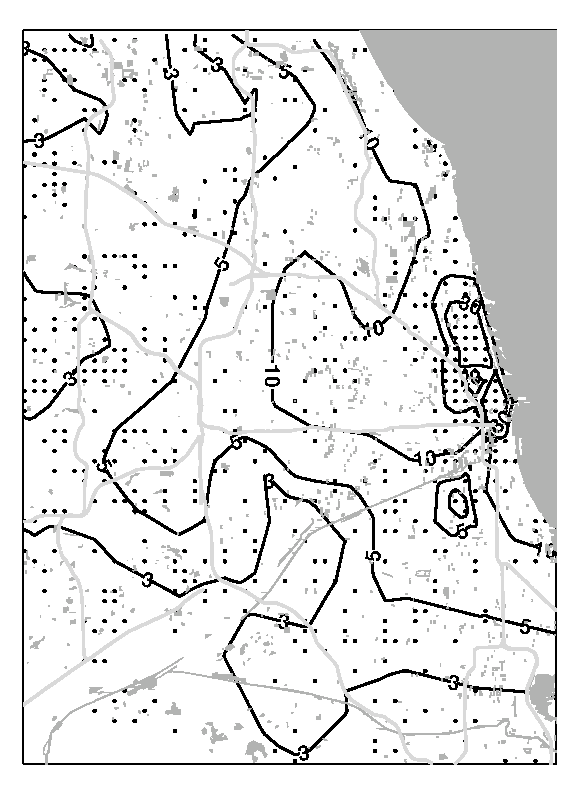
\epsfig{figure=chi25.eps, width=.32\textwidth}}\qquad
        \subfigure[Median]%
        {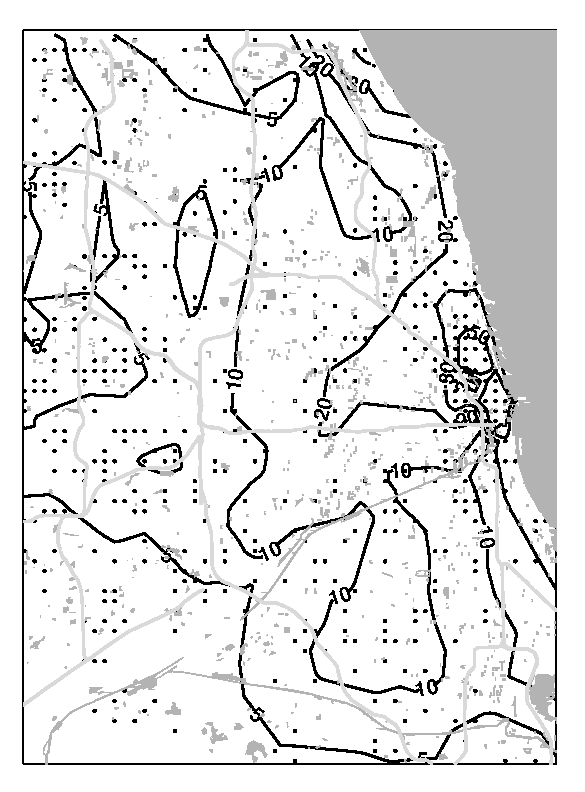
\epsfig{figure=chi50.eps, width=.32\textwidth}}\qquad
        \subfigure[Third quartile]%
        {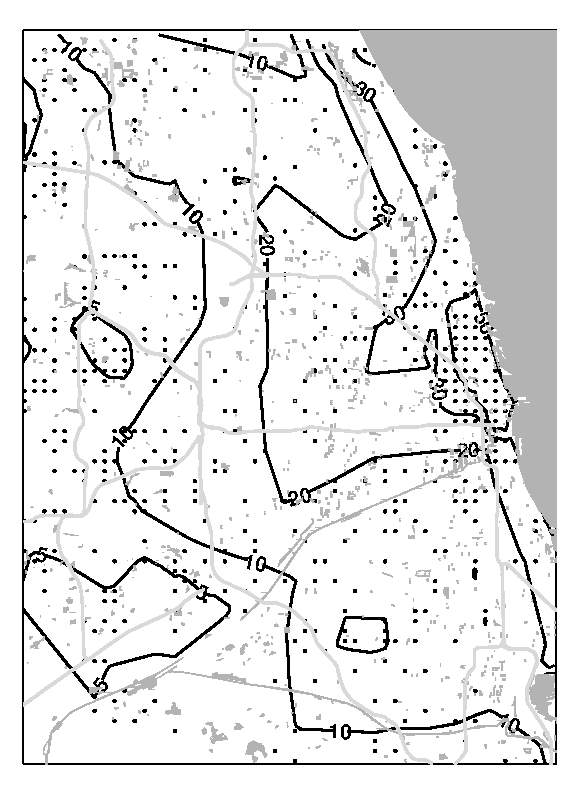
\epsfig{figure=chi75.eps, width=.32\textwidth}}}
\end{center}
\caption{Contours of Quartile Surfaces of Chicago Land Values.}
\end{figure}


\subsection{Chicago Land Values}
Our final example involves estimating a model for Chicago land values.
The data consist of 1194 vacant land sales occurring at 758 distinct sites
in the Chicago metropolitan area  during the period 1995--1997.
We take the sale price of the land
in dollars per square foot as $z_i$ and $(x_i,y_i)$. 
In Figures 5.2 we illustrate
three contour plots corresponding to fitted surfaces estimated by
solving the problem \eqref{eq.augtrirq} for the three
quartiles $\tau \in \{ .25, .50, .75\}$  of the land value distribution.
In these plots Lake Michigan appears in the upper right corner and the
Interstate highways are indicated in grey to provide landmarks
for the metropolitan area.  The central business district appears in
each of the plots as a closed contour of high land value
near the lake.  The scattered points in the plots indicate the locations
of the observed land sales used to fit the land value surfaces.
In each case the smoothing parameter $\lambda$  
is chosen, somewhat arbitrarily, to be .25.
This value is intermediate between the value selected by the 
SIC and AIC criteria  mentioned in Section 4.7 In our judgment 
SIC yields a somewhat oversmoothed fit, with $p_\lambda = 57$,
while AIC yields a a somewhat undersmoothed fit, with $p_\lambda = 220$,
for the median model.  Contours are labeled in dollars per square foot.  
We would like to emphasize that it may be advantageous in many smoothing
problems to estimate a family of conditional quantile curves, or surfaces,
since the commonly assumed independent and identically distributed  error model 
is rarely really plausible.
For land values, or annual temperatures, or snowfalls, it seems useful to
have some estimate of the way variability varies over the domain.


\begin{figure}[ht]
\begin{center}
\resizebox{\textwidth}{!}{
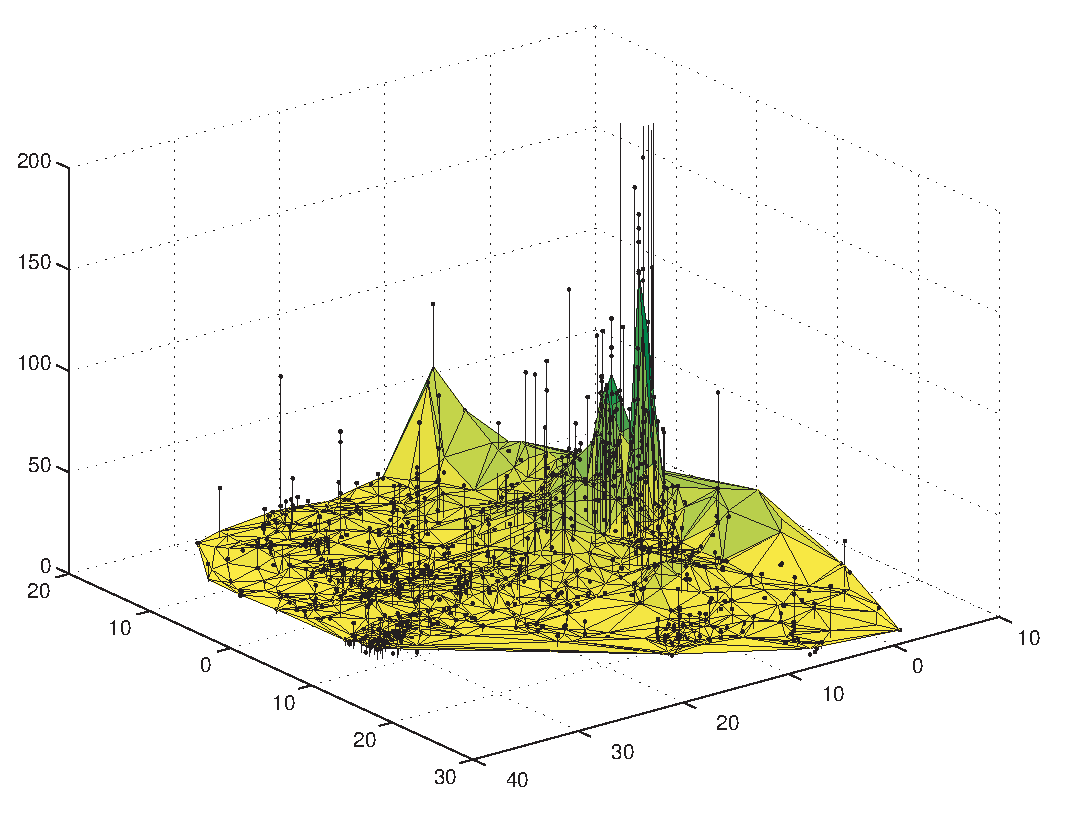
\includegraphics{chicago7.eps}}
\end{center}
\caption{Perspective Plot of Median Chicago Land Values.}
\end{figure}

The perspective plot of the median fit appearing in Figure~5.2
illustrates the ability of the total variation penalty to capture 
the sharp peaks of the Chicago land value surface. 
The figure depicts the responses lying above the fitted surface by
dots projected into the fitted surface.   As in the median contour
plot $\lambda$ is set equal to $0.25$. 
The five longest lines end without dots, indicating 
censored responses, prices so high that their inclusion and subsequent rescaling of the 
figure would render the plot trivial.  An important virtue of fitting quantile surfaces
to data of this sort is its lack of sensitivity to such extreme observations; points
that may need to be censored for plotting purposes, need not be censored for fitting
purposes.  Half of the data points are hidden beneath the surface.
The extreme skewness and heavy-tailedness in the response
can be seen from the following normal qqplot of the residuals.

\begin{figure}[ht]
\begin{center}
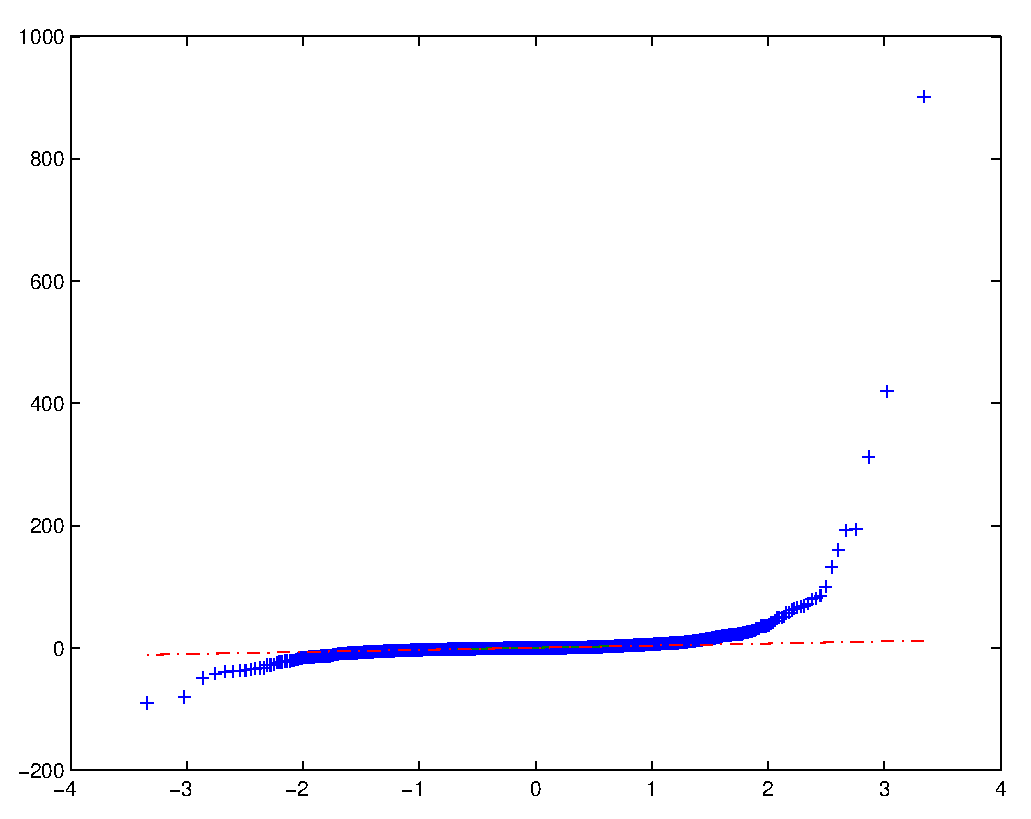
\includegraphics[width=9cm]{qqnorm.eps}
\end{center}
\caption{Normal QQ of Residuals from the Median Fit.}
\end{figure}

Among several possible refinements of this simple model
for land values, we note that it is quite straightforward to add
other covariates like the parcel size in a partially linear model formulation.
See \citeasnoun{KM.02} for further details on this approach.

\section{Conclusions}

We believe that regularization, or shrinkage, methods offer a
promising complementary approach to knot selection for triogram models.
Roughness penalties based on total variation seem particularly well-suited.
They satisfy natural equivariance requirements
and are computationally very attractive.
There are many possible lines of development for penalized triograms:
from fundamental questions about the geometric measure theory of
total variation of vector valued functions, 
to pragmatic issues of algorithmic design.
Further work is clearly necessary, but a strong {\it prima facie}
case has been made for the attractive features of total variation penalties
and their application to triogram estimation. 


\section{Acknowlegments}
A preliminary version of this  paper was presented at a conference 
in honor of George Judge held at the University of Illinois, May 1--2, 1999.
The research was partially supported by the NSF grant SES-99-11184, and by the 
Natural Sciences and Engineering Research Council of Canada.
The authors would like express their appreciation to 
Jana \Jureckova for the hospitality afforded them by the Department of 
Probability and Statistics of Charles University, to 
Steve Portnoy, Xuming He, and Hee-Seok Oh  for many helpful discussions, to Peter
Colwell and Henry Munneke for providing the Chicago land value data, and to an
anonymous referee who provided numerous suggestions that improved the presentation.

\bibliography{abbrev,gon1,pen}

\end{document}
